%!TEX root = ../../book_ML.tex
\chapter{$K$-lân cận}
\label{cha:knn}


Nếu con người có kiểu học ``nước đến chân mới nhảy'' thì machine
learning cũng có một thuật toán như vậy.


\section{Giới thiệu}


% \subsection{Một câu chuyện vui}

% Có một anh bạn chuẩn bị đến ngày thi cuối kỳ. Vì môn này được mở tài liệu khi
% thi nên anh ta không chịu ôn tập để hiểu ý nghĩa của từng bài học, mối liên hệ,
% và bản chất của vấn đề. Thay vào đó, anh thu thập tất cả các tài liệu trên lớp,
% bao gồm ghi chép bài giảng, các slides, bài tập về nhà, lời giải, cũng như đề
% thi của các năm trước. Cuối cùng, anh bạn của chúng ta thu thập được một chồng
% cao tài liệu để mang vào phòng thi.

% Vào ngày thi, anh tự tin mang chồng tài liệu vào phòng thi. Aha, đề này ít nhất
% mình phải được 8 điểm. Câu  giống hệt bài giảng trên lớp. Câu 2 giống hệt đề
% thi năm ngoái mà lời giải có trong tập tài liệu mua ở quán Photocopy. Câu 3 gần
% giống với bài tập về nhà. Câu 4 trắc nghiệm thậm chí cậu nhớ chính xác ba tài
% liệu có ghi đáp án. Câu cuối cùng, 1 câu khó nhưng anh đã từng nhìn thấy, chỉ là
% không nhớ ở đâu thôi.

% Kết quả cuối cùng, cậu ta được 4 điểm, vừa đủ điểm qua môn. Cậu làm chính xác
% câu 1 vì tìm được ngay trong tập ghi chú bài giảng. Câu 2 cũng tìm được đáp án
% nhưng lời giải của quán Photocopy sai! Câu ba thấy gần giống bài về nhà, chỉ
% khác mỗi một số thôi, cậu cho kết quả giống như thế luôn, vậy mà không được điểm
% nào. Câu 4 thì tìm được cả 3 tài liệu nhưng có hai trong đó cho đáp án A, cái
% còn lại cho B. Cậu chọn A và được điểm. Câu 5 thì không làm được dù còn tới 20
% phút, vì tìm mãi chẳng thấy đáp án đâu - nhiều tài liệu quá cũng mệt!!

% Không phải ngẫu nhiên mà tôi dành ra ba đoạn văn để kể về chuyện học hành của
% anh chàng kia. Hôm nay tôi xin trình bày về một phương pháp trong Machine
% Learning, được gọi là K-nearest neighbor (hay KNN), một thuật toán được xếp vào
% loại lazy (machine) learning (máy lười học). Thuật toán này khá giống với cách
% học/thi của anh bạn kém may mắn kia.

\index{$K$ lân cận -- $K$-nearest neighbor}
\index{KNN}
% \index{KNN, \textit{xem} K lân cận}
\subsection{K lân cận}
% \index{lazy learning}
\textit{K lân cận} (\textit{K-nearest neighbor} hay KNN) là một trong những
thuật toán học có giám sát đơn giản nhất. Khi huấn luyện, thuật toán này gần như
\textit{không học} một điều gì từ dữ liệu huấn luyện mà \textit{ghi nhớ} lại một
cách máy móc toàn bộ dữ liệu đó. Mọi tính toán được thực hiện khi tại pha kiểm
tra. KNN có thể được áp dụng vào các bài toán phân loại và hồi quy. KNN còn được
gọi là một thuật toán \textit{lười học},
\textit{instance-based}~\cite{aha1991instance}, hoặc \textit{memory-based
learning}.

% Có một vài khái niệm tương ứng người-máy như sau:

% |          Ngôn ngữ người         |    Ngôn ngữ Máy Học   | in Machine Learning |
% | --  --  --  --  --  --  --  --  --  --  --  --  --  --  --  -- -| --  --  --  --  --  --  --  --  --  --  -- -| --  --  --  --  --  --  --  --  --  -- -|
% | Câu hỏi                         | Điểm dữ liệu          | Data point          |
% | Đáp án                          | Đầu ra, nhãn          | Output, Label       |
% | Ôn thi                          | Huấn luyện            | Training            |
% | Tập tài liệu mang vào phòng thi | Tập dữ liệu tập huấn  | Training set        |
% | Đề thi                          | Tập dữ liểu kiểm tra  | Test set            |
% | Câu hỏi trong dề thi            | Dữ liệu kiểm tra      | Test data point     |
% | Câu hỏi có đáp án sai           | Nhiễu                 | Noise, Outlier      |
% | Câu hỏi gần giống               | Điểm dữ liệu gần nhất | Nearest Neighbor    |

% \index{bầu chọn theo đa số -- major voting}

% Trong bài toán phân loại, nhãn của một điểm dữ liệu mới được suy ra trực tiếp từ
% $K$ điểm dữ liệu gần nhất trong tập huấn luyện. Nhãn đó có thể được quyết định
% thông qua \textit{bầu chọn theo đa số} (\textit{major voting})trong số $K$ điểm
% gần nhất, hoặc nó có thể được suy ra bằng cách đánh trọng số khác nhau cho mỗi điểm đó rồi suy ra kết quả. Chi tiết sẽ được nêu trong mục
% tiếp theo. Trong bài toán hồi quy, đầu ra của một điểm dữ liệu sẽ bằng chính
% đầu ra của điểm dữ liệu đã biết gần nhất (trong trường hợp $K=1$), hoặc là trung
% bình có trọng số của đầu ra của những điểm gần nhất hay một mối quan hệ
% dựa trên các điểm gần nhất đó và khoảng cách tới chúng.

KNN là thuật toán đi tìm đầu ra của một điểm dữ liệu mới chỉ dựa trên thông tin của $K$ điểm dữ liệu gần nhất trong tập
huấn luyện. 
% ******************************************************************************
\begin{figure}[t]
    % caption on side     
    \floatbox[{\capbeside\thisfloatsetup{capbesideposition={right,top},capbesidewidth=7cm}}]{figure}[\FBwidth]
    {\caption{ 
    Ví dụ về 1NN. Các hình tròn là các điểm dữ liệu huấn luyện. Các hình khác
    màu thể hiện các lớp khác nhau. Các vùng nền thể hiện các điểm được phân
    loại vào lớp có màu tương ứng khi sử dựng 1NN (Nguồn:
    \href{https://en.wikipedia.org/wiki/K-nearest_neighbors_algorithm}{K-nearest
    neighbors algorithm  --  Wikipedia}, xem ảnh màu trong Hình~\ref{fig:6_1nn_c}).
    }
    \label{fig:6_1nn}}
    { % figure here
    % 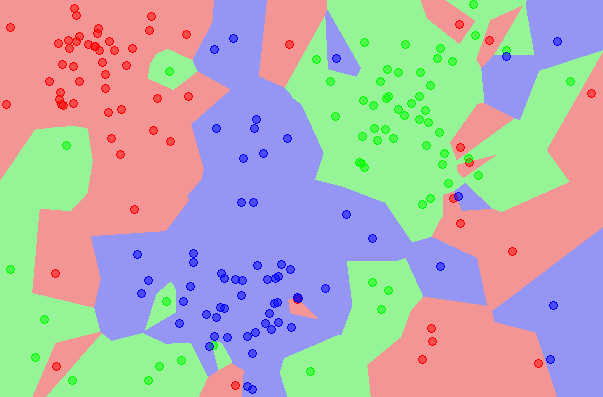
\includegraphics[width=.5\textwidth]{Chapters/03_SimpleML/6_knn/Map1NN.png}
    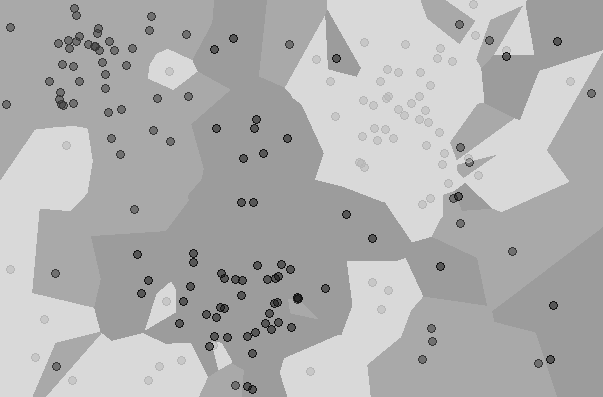
\includegraphics[width=.5\textwidth]{Chapters/03_SimpleML/6_knn/Map1NN_gray.png}
    }
\end{figure}
% ******************************************************************************


Hình~\ref{fig:6_1nn} mô tả một bài toán phân loại với ba nhãn: đỏ, lam, lục (xem ảnh màu trong Hình~\ref{fig:6_1nn_c}). Các
hình tròn nhỏ với màu khác nhau thể hiện dữ liệu huấn luyện của các nhãn khác
nhau. Các vùng màu nền khác nhau thể hiện ``lãnh thổ'' của mỗi nhãn. Nhãn của một điểm bất kỳ được xác định dựa trên nhãn của điểm gần nó nhất
trong tập huấn luyện. Trong hình này, có một vài vùng nhỏ xem lẫn vào các
vùng lớn hơn khác màu. Điểm này rất có thể là nhiễu. Các điểm dữ liệu kiểm tra gần khu vực điểm này nhiều khả năng sẽ bị phân loại sai.

Với KNN, mọi điểm trong tập
huấn luyện đều được mô hình mô tả một cách chính xác. Việc này khiến overfitting dễ xảy ra với KNN. 

Mặc dù có nhiều hạn chế, KNN vẫn là giải pháp đầu tiên nên nghĩ tới khi giải
quyết một bài toán machine learning. {Khi làm các bài toán machine
learning nói chung, không có mô hình đúng hay sai, chỉ có mô hình cho kết quả
tốt hơn. Chúng ta luôn cần một mô hình đơn giản để giải quyết bài toán, sau đó mới dần tìm cách tăng chất lượng của mô hình.}



% \subsection{Khoảng cách trong không gian vector}

% Trong không gian một chiều, khoảng cách giữa hai điểm là trị tuyệt đối giữa hiệu
% giá trị của hai điểm đó. Trong không gian nhiều chiều, khoảng cách giữa hai điểm
% có thể được định nghĩa bằng nhiều hàm số khác nhau, trong đó độ dài đường thằng
% nổi hai điểm chỉ là một trường hợp đặc biệt trong đó. Nhiều thông tin bổ ích
% (cho Machine Learning) có thể được tìm thấy tại
% \href{http://machinelearningcoban.com/math/#-norms-chuan}{Norms (chuẩn) của
% vector} trong tab \href{http://machinelearningcoban.com/math/}{Math}.




\section{Phân tích toán học}
% Thuật toán KNN rất dễ hiểu nên sẽ phần "Phân tích toán học" này sẽ chỉ có 3 câu.
% Tôi trực tiếp đi vào các ví dụ. Có một điều đáng lưu ý là KNN phải \textit{nhớ}
% tất cả các điểm dữ liệu training, việc này không được lợi về cả bộ nhớ và thời
% gian tính toán - giống như khi cậu bạn của chúng ta không tìm được câu trả lời
% cho câu hỏi cuối cùng.
Không có hàm mất mát hay bài toán tối ưu nào cần thực hiện trong quá trình
huấn luyện KNN. Mọi tính toán được tiến hành ở bước kiểm tra. Vì KNN ra quyết
định dựa trên các điểm gần nhất nên có hai vấn đề ta cần lưu tâm. Thứ nhất,
khoảng cách được định nghĩa như thế nào. Thứ hai, cần phải tính toán khoảng cách
như thế nào cho hiệu quả.

Với vấn đề thứ nhất, mỗi điểm dữ liệu được thể hiện bằng một vector đặc trưng,
khoảng cách giữa hai điểm chính là khoảng cách giữa hai vector đó. Có nhiều loại khoảng cách khác nhau tuỳ vào bài toán, nhưng khoảng cách được sử dụng nhiều nhất là khoảng cách Euclid (xem Mục~\ref{sec:2_norm}). 

\index{quy mô lớn -- large-scale}

Vấn đề thứ hai cần được lưu tâm hơn, đặc biệt với {các bài toán với tập huấn
luyện lớn và vector dữ liệu có kích thước lớn}. Giả sử các vector huấn luyện là
các cột của ma trận $\bX\in \R^{d\times N}$ với $d$ và $N$ lớn. KNN sẽ phải tính khoảng cách từ một điểm dữ liệu mới $\bz \in \R^{d}$ đến toàn bộ $N$ điểm
dữ liệu đã cho và chọn ra $K$ khoảng cách nhỏ nhất. Nếu không có cách tính hiệu
quả, khối lượng tính toán sẽ rất lớn.

Tiếp theo, chúng ta cùng thực hiện một vài phân tích toán học để tìm ra một cách hiệu quả để tính các khoảng cách. Ở đây khoảng cách được xem xét là khoảng cách Euclid.
% \subsection{Một cách hiệu quả để tính khoảng cách}
\subsubsection{Khoảng cách từ một điểm tới từng điểm trong một tập hợp}
Khoảng cách Euclid từ một điểm $\bz$ tới một điểm $\bx_i$ trong tập
huấn luyện được định nghĩa bởi $\|\bz - \bx_i\|_2$. Người ta thường dùng bình phương khoảng cách Euclid $\|\bz -\bx_i\|_2^2$ để tránh phép tính căn bậc hai. Việc bình phương này không ảnh hưởng tới thứ tự của các khoảng cách. Để ý rằng
\begin{equation}
\label{eqn:6_dist}
    \|\bz - \bx_i\|_2^2 = (\bz - \bx_i)^T(\bz - \bx_i) = \|\bz\|_2^2 +
        \|\bx_i\|_2^2 - 2\bx_i^T\bz 
\end{equation}
Để tìm ra $\bx_i$ gần với $\bz$ nhất, số hạng đầu tiên
có thể được bỏ qua. Hơn nữa, nếu có nhiều điểm dữ liệu trong tập kiểm tra, các
giá trị $\|\bx_i\|_2^2$ có thể được tính và lưu trước vào bộ nhớ. Khi đó, ta chỉ
cần tính các tích vô hướng $\bx_i^T\bz$.

Để thấy rõ hơn, chúng ta cùng làm một ví dụ trên Python. Trước hết, chọn $d$ và
$N$ là các giá trị lớn và khai báo ngẫu nhiên $\bX$ và $\bz$. Khi lập trình Python, cần lưu ý rằng chiều thứ nhất thường chỉ thứ tự của điểm dữ liệu.
\begin{lstlisting}[language=Python]
from __future__ import print_function 
import numpy as np 
from time import time # for comparing runing time 
d, N = 1000, 10000 # dimension, number of training points 
X = np.random.randn(N, d) # N d-dimensional points 
z = np.random.randn(d) 
\end{lstlisting}

Tiếp theo, ta viết ba hàm số: 
\begin{enumerate}

    \item \pythoninline{dist_pp(z, x)} tính bình phương khoảng cách Euclid giữa \pythoninline{z} và \pythoninline{x}. Hàm này tính hiệu $\bz - \bx$ rồi lấy bình phương $\ell_2$ norm của nó. 


    \item \pythoninline{dist_ps_naive(z, X)} tính bình phương khoảng cách giữa
    \pythoninline{z} và mỗi {hàng} của \pythoninline{X}. Trong hàm này,
    các khoảng cách được xây dựng dựa trên việc tính từng giá trị
    \pythoninline{dist_pp(z, X[i])}. 

    \item \pythoninline{dist_ps_fast(z, X)} tính bình phương khoảng cách giữa
    \pythoninline{z} và mỗi {hàng} của \pythoninline{X}, tuy nhiên, kết
    quả được tính dựa trên đẳng thức~\eqref{eqn:6_dist}. Ta cần tính tổng bình phương các phần tử của mỗi điểm dữ liệu trong \pythoninline{X} và tính tích \pythoninline{X.dot(z)}
\end{enumerate}

Đoạn code dưới đây thể hiện hai cách tính khoảng cách từ một điểm
\pythoninline{z} tới một tập hợp điểm \pythoninline{X}.
Kết quả và thời gian chạy của mỗi hàm được in ra để so sánh. 
% \newpage 

\begin{lstlisting}[language=Python]
# naively compute square distance between two vector 
def dist_pp(z, x): 
    d = z - x.reshape(z.shape) # force x and z to have the same dims 
    return np.sum(d*d)

# from one point to each point in a set, naive 
def dist_ps_naive(z, X):
    N = X.shape[0]
    res = np.zeros((1, N)) 
    for i in range(N):
        res[0][i] = dist_pp(z, X[i])
    return res 
\end{lstlisting}
\begin{lstlisting}[language=Python]
# from one point to each point in a set, fast
def dist_ps_fast(z, X):
    X2 = np.sum(X*X, 1) # square of l2 norm of each X[i], can be precomputed
    z2 = np.sum(z*z) # square of l2 norm of z 
    return X2 + z2 - 2*X.dot(z) # z2 can be ignored

t1 = time() 
D1 = dist_ps_naive(z, X)
print('naive point2set, running time:', time() - t1, 's')

t1 = time() 
D2 = dist_ps_fast(z, X)
print('fast point2set , running time:', time() - t1, 's')
print('Result difference:', np.linalg.norm(D1 - D2))
\end{lstlisting}

\kq 
\begin{lstlisting}[language=Python]
naive point2set, running time: 0.0932548046112 s
fast point2set , running time: 0.0514178276062 s
Result difference: 2.11481965531e-11
\end{lstlisting}

Kết quả chỉ ra rằng hàm \pythoninline{dist_ps_fast(z, X)} chạy nhanh hơn gần
gấp đôi so với hàm \pythoninline{dist_ps_naive(z, X)}. Tỉ lệ này còn lớn hơn
khi kích thước dữ liệu tăng lên và \pythoninline{X2} được tính từ trước. Quan trọng hơn, sự chênh lệch nhỏ giữa kết quả của hai cách tính chỉ ra rằng \pythoninline{dist_ps_fast(z, X)} nên được ưu tiên hơn.

\subsubsection{Khoảng cách giữa từng cặp điểm trong hai tập hợp}
Thông thường, tập kiểm tra bao gồm nhiều điểm dữ liệu tạo thành một ma trận
$\bZ$. Ta phải tính từng cặp khoảng cách giữa mỗi điểm trong tập kiểm tra và một
điểm trong tập huấn luyện. Nếu mỗi tập có 1000 phần tử, có một triệu khoảng cách
cần tính. Nếu không có phương pháp tính hiệu quả, thời gian thực hiện sẽ rất dài.

Đoạn code dưới đây thể hiện hai phương pháp tính bình phương khoảng cách giữa
các cặp điểm trong hai tập điểm. Phương pháp thứ nhất sử dụng một vòng
\pythoninline{for} tính khoảng cách từ từng điểm trong tập thứ nhất đến tất cả
các điểm trong tập thứ hai thông qua hàm
\pythoninline{dist_ps_fast(z, X)} ở trên. Phương pháp thứ hai tiếp tục sử
dụng~\eqref{eqn:6_dist} cho trường hợp tổng quát.


\begin{lstlisting}[language=Python]
Z = np.random.randn(100, d)
# from each point in one set to each point in another set, half fast 
def dist_ss_0(Z, X):
    M, N = Z.shape[0], X.shape[0]
    res = np.zeros((M, N))
    for i in range(M):
        res[i] = dist_ps_fast(Z[i], X)
    return res 
\end{lstlisting}
\begin{lstlisting}[language=Python]
# from each point in one set to each point in another set, fast 
def dist_ss_fast(Z, X):
    X2 = np.sum(X*X, 1) # square of l2 norm of each ROW of X
    Z2 = np.sum(Z*Z, 1) # square of l2 norm of each ROW of Z
    return Z2.reshape(-1, 1) + X2.reshape(1, -1) - 2*Z.dot(X.T)

t1 = time() 
D3 = dist_ss_0(Z, X)
print('half fast set2set running time:', time() - t1, 's')
t1 = time() 
D4 = dist_ss_fast(Z, X)
print('fast set2set  running time', time() - t1, 's')
print('Result difference:', np.linalg.norm(D3 - D4))
\end{lstlisting}
\kq
\begin{lstlisting}[language=Python]
half fast set2set running time: 4.33642292023 s
fast set2set  running time 0.0583250522614 s
Result difference: 9.93586539607e-11
\end{lstlisting}
Điều này chỉ ra rằng hai cách tính cho kết quả chênh lệch nhau không đáng kể.
Trong khi đó \pythoninline{dist_ss_fast(Z, X)} chạy nhanh hơn
\pythoninline{dist_ss_0(Z, X)} nhiều lần. 

Khi làm việc trên python, chúng ta có thể sử dụng hàm
\pythoninline{cdist} (\url{https://goo.gl/vYMnmM}) trong
\pythoninline{scipy.spatial.distance}, hoặc hàm
\pythoninline{pairwise_distances} (\url{https://goo.gl/QK6Zyi}) trong
\pythoninline{sklearn.metrics.pairwise}. Các hàm này giúp tính khoảng cách từng 
cặp điểm trong hai tập hợp khá hiệu quả. Phần còn lại của chương này sẽ trực
tiếp sử dụng thư viện scikit-learn cho KNN. Việc viết lại thuật toán này không
quá phức tạp khi đã có một hàm tính khoảng cách hiệu quả. 

Bạn đọc có thể tham khảo thêm bài báo~\cite{johnson2017billion} về cách thực
hiện KNN trên  và mã nguồn tại
\url{https://github.com/facebookresearch/faiss}.



\section{Ví dụ trên cơ sở dữ liệu Iris}

\begin{figure}[t]
\centering
    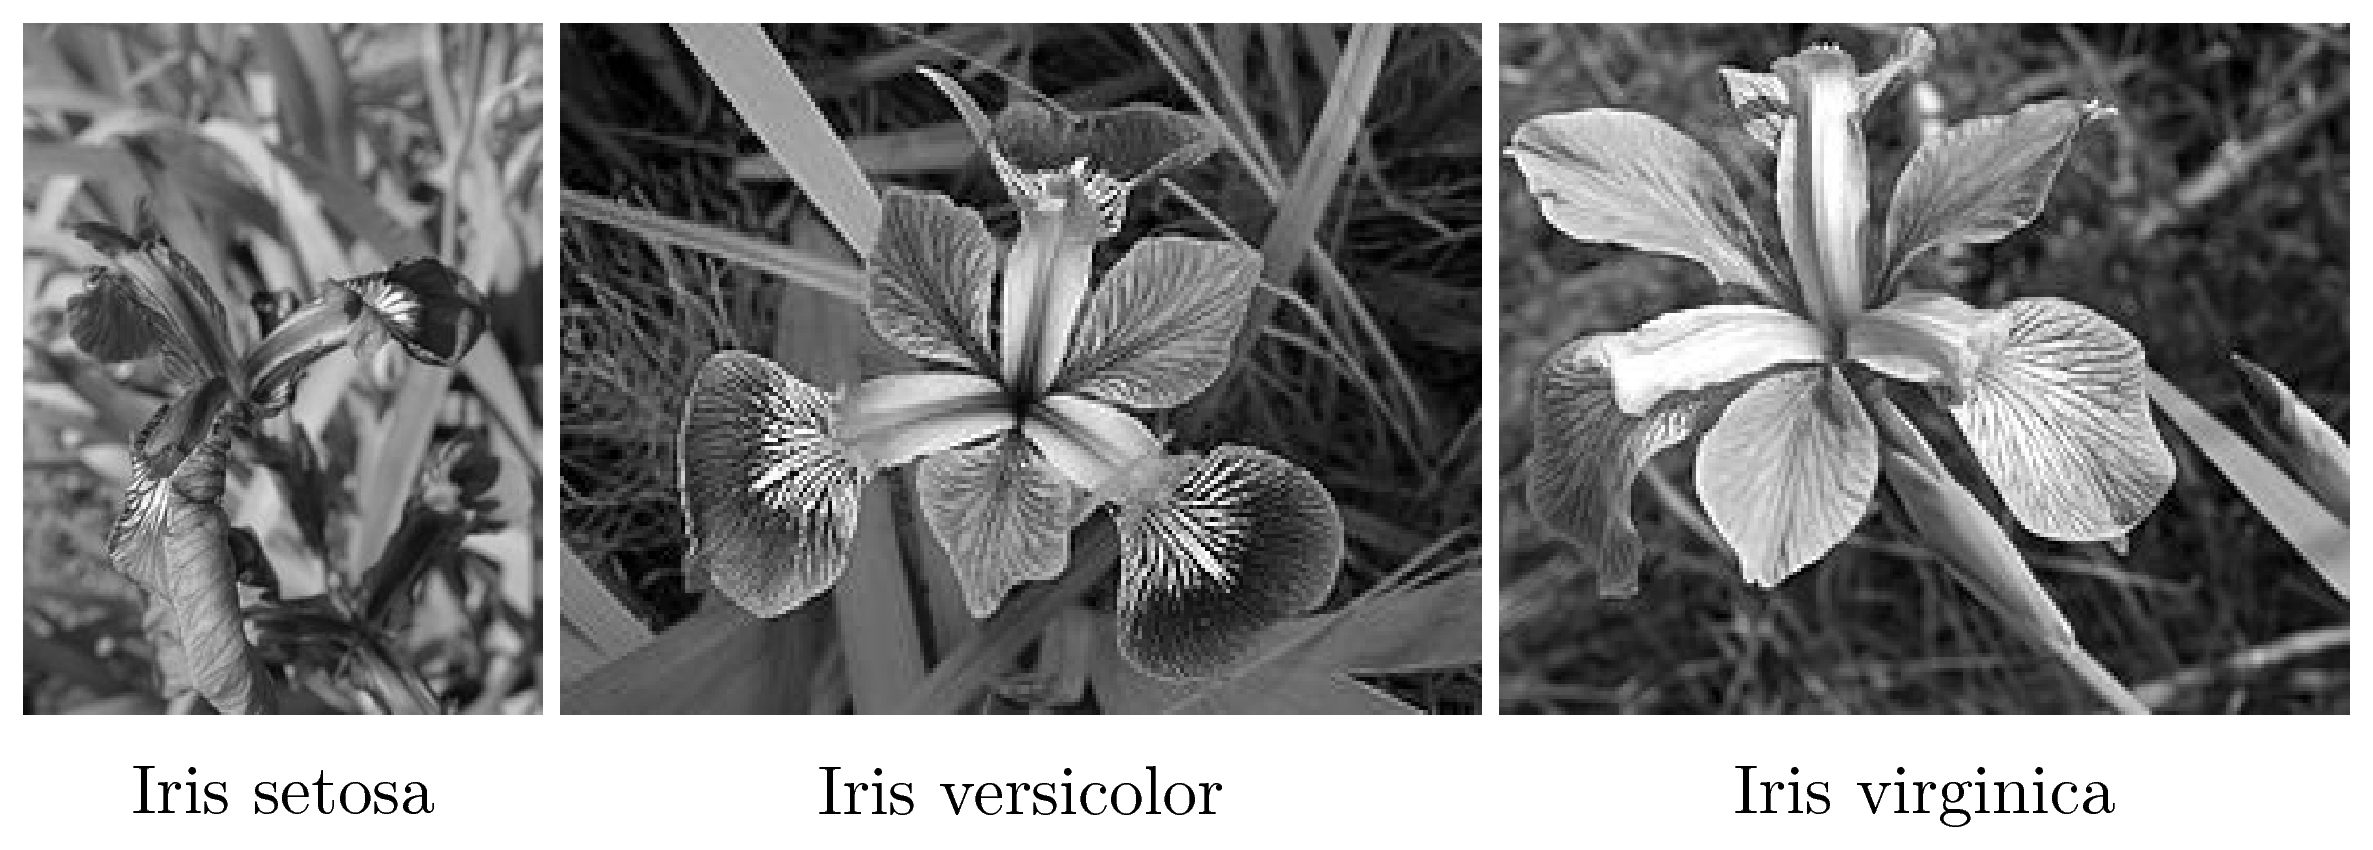
\includegraphics[width = \textwidth]{Chapters/03_SimpleML/6_knn/iris_gray.png}
    \caption[]{Ba loại hoa lan trong bộ cơ sở dữ liệu hoa Iris (xem ảnh màu trong Hình~\ref{fig:6_iris_c}).}
    \label{fig:6_iris}
\end{figure}


\subsection{Bộ cơ sở dữ liệu hoa Iris}

Bộ dữ liệu hoa Iris (\url{https://goo.gl/eUy83R}) là một bộ dữ liệu nhỏ. Bộ dữ
liệu này bao gồm thông tin của ba nhãn hoa Iris khác nhau: Iris setosa, Iris
virginica và Iris versicolor. Mỗi nhãn chứa thông tin của 50 bông hoa với dữ
liệu là bốn thông tin: chiều dài, chiều rộng đài hoa, và chiều dài,
chiều rộng cánh hoa. Hình~\ref{fig:6_iris} là ví dụ về hình ảnh của ba
loại hoa. Chú ý rằng các điểm dữ liệu không phải là các bức ảnh mà chỉ là một
vector đặc trưng bốn chiếu gồm các thông tin ở trên.

% \begin{figure}[t]
% \centering
%     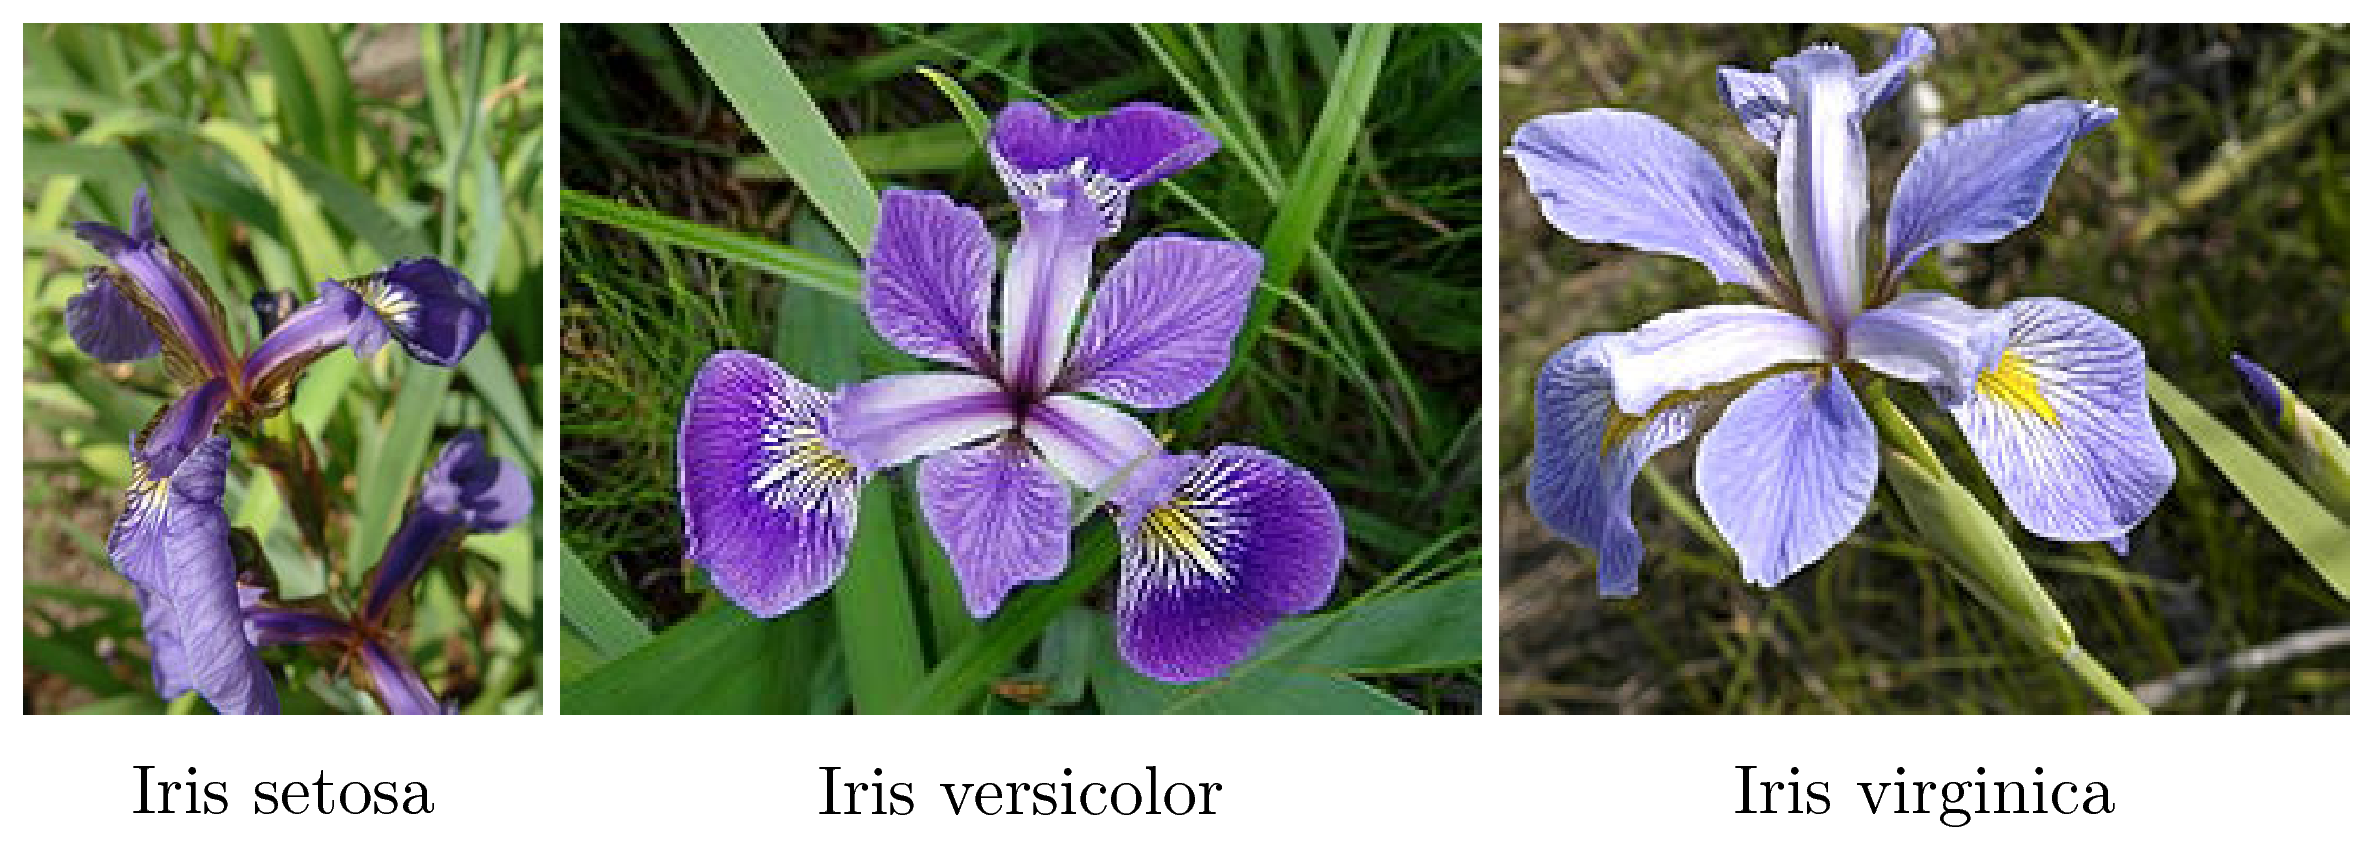
\includegraphics[width = \textwidth]{Chapters/03_SimpleML/6_knn/iris.png}
%     \caption[]{Ba loại hoa lan trong bộ cơ sở dữ liệu hoa Iris.}
%     \label{fig:6_iris}
% \end{figure}

% <div class="imgcap">
% <img src ="/assets/knn/iris.png" align = "center" width="800">
% <div class="thecap"> Ví dụ về Iris flower dataset (Nguồn: <a href = "https://en.wikipedia.org/wiki/Iris_flower_data_set">Wikipedia</a>) <br></div>
% </div>

% Bộ dữ liệu nhỏ này thường được sử dụng trong nhiều thuật toán Machine Learning
% trong các lớp học. Tôi sẽ giải thích lý do không chọn MNIST vào phần sau.



\subsection{Thí nghiệm}


Trong phần này, 150 điểm dữ liệu được tách thành tập huấn luyện và tập kiểm tra.
KNN dựa vào trông tin trong tập huấn luyện để dự đoán mỗi dữ liệu trong tập kiểm
tra tương ứng với loại hoa nào. Kết quả này được đối chiếu với đầu ra thực sự
để đánh giá hiệu quả của KNN.

Trước tiên, chúng ta cần khai báo vài thư viện. Bộ dữ liệu hoa Iris có sẵn trong
thư viện scikit-learn.

\begin{lstlisting}[language=Python]
from __future__ import print_function 
import numpy as np
from sklearn import neighbors, datasets
from sklearn.model_selection import train_test_split # for splitting data 
from sklearn.metrics import accuracy_score      # for evaluating results

iris = datasets.load_iris()
iris_X = iris.data
iris_y = iris.target
\end{lstlisting}

Tiếp theo, 130 mẫu dữ liệu được lấy ra ngẫu nhiên tạo thành tập huấn luyện, 20 mẫu còn lại được dùng để kiểm tra.
% \newpage 

\begin{lstlisting}[language=Python]
print('Labels:', np.unique(iris_y))

# split train and test 
np.random.seed(7) 
X_train, X_test, y_train, y_test = train_test_split(iris_X, iris_y, test_size=130)
print('Training size:', X_train.shape[0], ', test size:', X_test.shape[0])
\end{lstlisting}
\begin{lstlisting}
Labels: [0 1 2]
Training size: 20 , test size: 130
\end{lstlisting}

Dòng \pythoninline{np.random.seed(7)} để đảm bảo kết quả chạy ở các lần khác nhau là giống nhau. Có thể thay 7 bằng một số tự
nhiên 32 bit bất kỳ. 

\subsubsection{Kết quả với 1NN}
Tới đây, ta trực tiếp sử dụng thư viện scikit-learn cho KNN. Xét ví dụ đầu tiên
với $K = 1$.

\begin{lstlisting}[language=Python]
model = neighbors.KNeighborsClassifier(n_neighbors = 1, p = 2)
model.fit(X_train, y_train)
y_pred = model.predict(X_test)
print("Accuracy of 1NN: %.2f %%" %(100*accuracy_score(y_test, y_pred)))
\end{lstlisting}
\kq
\begin{lstlisting}[language=Python]
Accuracy of 1NN: 92.31 %
\end{lstlisting}

Kết quả thu được là 92.31\% (tỉ lệ số mẫu được phân loại chính xác trên tổng số
mẫu). Ở đây, \pythoninline{n_neighbors = 1} chỉ ra rằng chỉ điểm gần nhất được
lựa chọn, tức $K = 1$, \pythoninline{p = 2} chính là $\ell_2$ norm để tính
khoảng cách. Bạn đọc có thể thử với \pythoninline{p = 1} tương ứng với khoảng
cách $\ell_1$ norm.





% \subsubsection{Tách training và test sets}
% Giả sử chúng ta muốn dùng 50 điểm dữ liệu cho test set, 100 điểm còn lại cho
% training set. Scikit-learn có một hàm số cho phép chúng ta ngẫu nhiên lựa chọn
% các điểm này, như sau:


% \begin{lstlisting}[language=Python]
% from sklearn.model_selection import train_test_split
% X_train, X_test, y_train, y_test = train_test_split(
%      iris_X, iris_y, test_size=50)

% print "Training size: %d" %len(y_train)
% print "Test size    : %d" %len(y_test)
% \end{lstlisting}
% \begin{lstlisting}[language=Python]
% Training size: 100
% Test size    : 50
% \end{lstlisting}


% Sau đây, tôi trước hết xét trường hợp đơn giản K = 1, tức là với mỗi điểm test
% data, ta chỉ xét 1 điểm training data gần nhất và lấy label của điểm đó để dự
% đoán cho điểm test này.


% \begin{lstlisting}[language=Python]
% clf = neighbors.KNeighborsClassifier(n_neighbors = 1, p = 2)
% clf.fit(X_train, y_train)
% y_pred = clf.predict(X_test)

% print "Print results for 20 test data points:"
% print "Predicted labels: ", y_pred[20:40]
% print "Ground truth    : ", y_test[20:40]
% \end{lstlisting}
% \begin{lstlisting}[language=Python]
% Print results for first 20 test data points:
% Predicted labels:  [2 1 2 2 1 2 2 0 2 0 2 0 1 0 0 2 2 0 2 0]
% Ground truth    :  [2 1 2 2 1 2 2 0 2 0 1 0 1 0 0 2 1 0 2 0]
% \end{lstlisting}

% <a name = "ground-truth"></a>
% Kết quả cho thấy label dự đoán gần giống với label thật của test data, chỉ có 2
% điểm trong số 20 điểm được hiển thị có kết quả sai lệch. Ở đây chúng ta làm quen
% với khái niệm mới: \textit{ground truth}. Một cách đơn giản, \textit{ground
% truth} chính là nhãn/label/đầu ra \textit{thực sự} của các điểm trong test data.
% Khái niệm này được dùng nhiều trong Machine Learning, hy vọng lần tới các bạn
% gặp thì sẽ nhớ ngay nó là gì.



% \subsubsection{Phương pháp đánh giá (evaluation method)}
% Để đánh giá độ chính xác của thuật toán KNN classifier này, chúng ta xem xem có
% bao nhiêu điểm trong test data được dự đoán đúng. Lấy số lượng này chia cho tổng
% số lượng trong tập test data sẽ ra độ chính xác. Scikit-learn cung cấp hàm số
% \href{http://scikit-learn.org/stable/modules/generated/sklearn.metrics.accuracy_score.html}{\pythoninline{accuracy_score}} để
% thực hiện công việc này.


% \begin{lstlisting}[language=Python]
% from sklearn.metrics import accuracy_score
% print "Accuracy of 1NN: %.2f %%" %(100*accuracy_score(y_test, y_pred))
% \end{lstlisting}

% \begin{lstlisting}[language=Python]
% Accuracy of 1NN: 94.00 %
% \end{lstlisting}


% 1NN đã cho chúng ta kết quả là 94\%, không tệ! Chú ý rằng đây là một cơ sở dữ
% liệu dễ vì chỉ với dữ liệu ở hai cột cuối cùng, chúng ta đã có thể suy ra quy
% luật. Trong ví dụ này, tôi sử dụng \pythoninline{p = 2} nghĩa là khoảng cách ở
% đây được tính là khoảng cách theo
% \href{http://machinelearningcoban.com/math/#norm2}{$\ell_2$ norm}. Các bạn cũng có thể
% thử bằng cách thay \pythoninline{p = 1} cho
% \href{http://machinelearningcoban.com/math/#norm0}{norm 1}, hoặc các gía trị
% \pythoninline{p} khác cho norm khác. (Xem thêm
% \href{http://scikit-learn.org/stable/modules/generated/sklearn.neighbors.KNeighborsClassifier.html}{sklearn.neighbors.KNeighborsClassifier})

\subsubsection{Kết quả với 7NN}
\index{bầu chọn đa số -- major voting}
Như đã đề cập, 1NN rất dễ gây ra overfitting. Để hạn chế việc này, ta có thể
tăng lượng điểm lân cận lên, ví dụ bảy điểm, kết quả được xác định dựa trên đa
số.

\begin{lstlisting}[language=Python]
model = neighbors.KNeighborsClassifier(n_neighbors = 7, p = 2)
model.fit(X_train, y_train)
y_pred = model.predict(X_test)

print("Accuracy of 7NN with major voting: %.2f %%" %(100*accuracy_score(y_test, y_pred)))

\end{lstlisting}
\kq 
\begin{lstlisting}[language=Python]
Accuracy of 7NN with major voting: 93.85 %
\end{lstlisting}

Nhận thấy rằng khi sử dụng nhiều điểm lân cận hơn, độ chính xác đã tăng lên. Phương pháp dựa trên đa số trong lân cận còn được gọi là \textit{bầu chọn đa số}.

% \begin{lstlisting}[language=Python]
% clf = neighbors.KNeighborsClassifier(n_neighbors = 10, p = 2)
% clf.fit(X_train, y_train)
% y_pred = clf.predict(X_test)

% print "Accuracy of 10NN with major voting: %.2f %%" %(100*accuracy_score(y_test, y_pred))
% \end{lstlisting}
% \begin{lstlisting}[language=Python]
% Accuracy of 10NN with major voting: 98.00 %
% \end{lstlisting}


% Kết quả đã tăng lên 98%, rất tốt!



\subsubsection{Đánh trọng số cho các điểm lân cận}
Trong kỹ thuật bầu chọn đa số phía trên, các điểm trong bảy điểm gần nhất đều có
vai trò như nhau và giá trị ``lá phiếu'' của mỗi điểm này cũng như nhau. Cách bầu chọn này có thể thiếu công bằng vì các điểm gần hơn nên có tầm ảnh hưởng lớn hơn. Để thực hiện việc này, ta chỉ cần đánh trọng số khác nhau cho từng điểm trong bảy điểm gần nhất này. Cách
đánh trọng số phải thoả mãn điều kiện điểm lân cận hơn được đánh trọng số cao hơn. Một cách đơn giản là lấy nghịch đảo của khoảng
cách tới điểm lân cận. Trong trường hợp tồn tại khoảng cách bằng không, tức điểm kiểm tra trùng với một điểm huấn luyện, ta trực tiếp lấy đầu ra của điểm huấn luyện đó.

Để thực hiện việc này trong scikit-learn, ta chỉ cần gán
\pythoninline{weights = 'distance'}. Giá trị mặc định của
\pythoninline{weights} là \pythoninline{'uniform'}, tương ứng với việc coi tất
cả các điểm lân cận có giá trị bằng nhau như trong bầu chọn đa số.

\begin{lstlisting}[language=Python]
model = neighbors.KNeighborsClassifier(n_neighbors = 7, p = 2, \
    weights = 'distance')
model.fit(X_train, y_train)
y_pred = model.predict(X_test)

print("Accuracy of 7NN (1/distance weights): %.2f %%" %(100*accuracy_score(y_test, y_pred)))
\end{lstlisting}
\kq
\begin{lstlisting}[language=Python]
Accuracy of 7NN (1/distance weights): 94.62 %
\end{lstlisting}
% \begin{lstlisting}[language=Python]
% clf = neighbors.KNeighborsClassifier(n_neighbors = 10, p = 2, weights = 'distance')
% clf.fit(X_train, y_train)
% y_pred = clf.predict(X_test)

% print "Accuracy of 10NN (1/distance weights): %.2f %%" %(100*accuracy_score(y_test, y_pred))
% \end{lstlisting}
% \begin{lstlisting}[language=Python]
% Accuracy of 10NN (1/distance weights): 100.00 %
% \end{lstlisting}


Độ chính xác tiếp tục được tăng lên. 

\subsubsection{KNN với trọng số tự định nghĩa}
Ngoài hai cách đánh trọng số \pythoninline{weights =
`uniform'} và \pythoninline{weights = `distance'}, scikit-learn còn cung
cấp cách đánh trọng số tùy chọn. Ví dụ, một cách
đánh trọng số phổ biến khác thường được dùng là
\begin{equation*}
w_i = \exp \left( \frac{-\|\mathbf{z} - \mathbf{x}_i\|_2^2}{\sigma^2}
\right)
\end{equation*}
trong đó $w_i$ là trọng số của điểm gần thứ $i$ ($\bx_i$) của điểm dữ liệu
đang xét $\mathbf{z}$, $\sigma$ là một số dương. Hàm số này cũng
thỏa mãn
điều kiện điểm càng gần $\mathbf{x}$ thì trọng số càng cao (cao nhất bằng 1).
Với hàm số này, ta có thể lập trình như sau:


\begin{lstlisting}[language=Python]
def myweight(distances):
    sigma2 = .4 # we can change this number
    return np.exp(-distances**2/sigma2)

model = neighbors.KNeighborsClassifier(n_neighbors = 7, p = 2, weights = myweight)
model.fit(X_train, y_train)
y_pred = model.predict(X_test)

print("Accuracy of 7NN (customized weights): %.2f %%"
 (100*accuracy_score(y_test, y_pred)))
\end{lstlisting}
\kq
\begin{lstlisting}[language=Python]
Accuracy of 7NN (customized weights): 95.38 %
\end{lstlisting}

Kết quả tiếp tục tăng lên một chút. Với từng bài toán, chúng ta có thể
thay các thuộc tính của KNN bằng các giá trị khác nhau và chọn ra giá trị tốt
nhất thông qua xác thực chéo (xem Mục~\ref{ssec:crosvalid}).

% Trong trường hợp này, kết quả tương đương với kỹ thuật major voting. Để đánh giá
% chính xác hơn kết quả của KNN với K khác nhau, cách định nghĩa khoảng cách khác
% nhau và cách đánh trọng số khác nhau, chúng ta cần thực hiện quá trình trên với
% nhiều cách chia dữ liệu \textit{training} và \textit{test} khác nhau rồi lấy kết
% quả trung bình, vì rất có thể dữ liệu phân chia trong 1 trường hợp cụ thể là rất
% tốt hoặc rất xấu (bias). Đây cũng là cách thường được dùng khi đánh giá hiệu
% năng của một thuật toán cụ thể nào đó.



\section{Thảo luận}



\subsection{KNN cho bài toán hồi quy}
Với bài toán hồi quy, chúng ta cũng hoàn toàn có thể sử dụng phương pháp
tương tự: đầu ra của một điểm được xác định dựa trên đầu ra của các điểm lân cận
và khoảng cách tới chúng. Giả sử $\bx_1, \dots, \bx_K$ là $K$ điểm lân cận của
một điểm dữ liệu $\bz$ với đầu ra tương ứng là $y_1, \dots, y_K$. Giả sử các
trọng số ứng với các lân cận này là $w_1, \dots, w_K$. Kết quả dự đoán
đầu ra của $\bz$ có thể được xác định bởi
\begin{equation}
\displaystyle
    \frac{w_1 y_1 + w_2 y_2 + \dots + w_Kw_K}{w_1 + w_2 + \dots + w_K}
\end{equation}
Hình~\ref{fig:6_knn_reg} là một ví dụ về KNN cho hồi quy với $K = 5$,
sử dụng hai cách đánh trọng số khác nhau. Ta có thể thấy rằng
\pythoninline{weights = 'distance'} có xu hướng gây ra overfitting. 

\begin{figure}[t]
\centering
    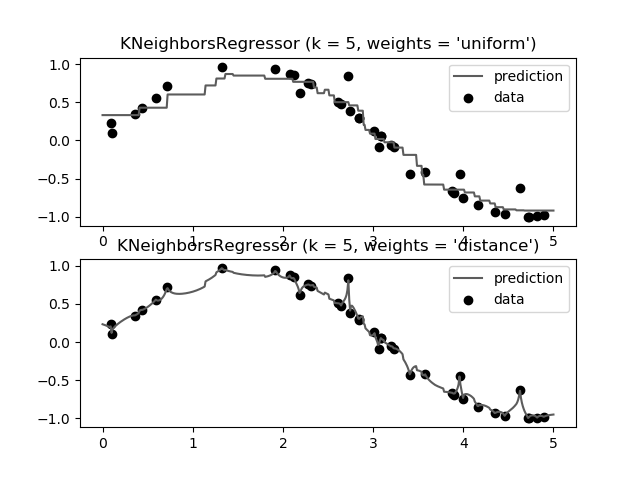
\includegraphics[width =
    .7\textwidth]{Chapters/03_SimpleML/6_knn/sphx_glr_plot_regression_001_gray.png}
    \caption[]{KNN cho bài toán hồi quy (Nguồn:
    \textit{Nearest neighbors regression -- scikit-learn} -- \url{https://goo.gl/9VyBF3}).}
    \label{fig:6_knn_reg}
\end{figure}
% \begin{figure}[t]
%     % caption on side     



%     \floatbox[{\capbeside\thisfloatsetup{capbesideposition={right,top},capbesidewidth=3cm}}]{figure}[\FBwidth]
%     {\caption{ 
%     KNN cho bài toán Regression (Nguồn:
%     \href{https://goo.gl/9VyBF3}{Nearest Neighbors regression  --  scikit-learn}).
%     }
%     \label{fig:6_knn_reg}}
%     { % figure here
%     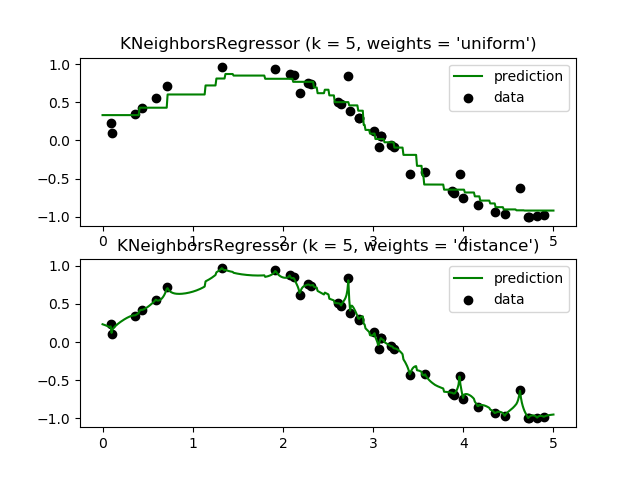
\includegraphics[width=.75\textwidth]{Chapters/03_SimpleML/6_knn/sphx_glr_plot_regression_001.png}
%     }
% \end{figure}


% <div class="imgcap">
% <img src ="http://scikit-learn.org/stable/_images/sphx_glr_plot_regression_001.png" align = "center">
% <div class="thecap"> KNN cho bài toán Regression  (Nguồn: <a href = "http://scikit-learn.org/stable/auto_examples/neighbors/plot_regression.html#sphx-glr-auto-examples-neighbors-plot-regression-py">Nearest Neighbors regression</a>) <br></div>
% </div>



% \subsection{Chuẩn hóa dữ liệu}
% Khi có một thuộc tính trong vector đặc trưng lớn hơn các thuộc tính khác rất
% nhiều, chẳng hạn ví dụ thay vì đo bằng cm thì một kết quả lại tính bằng mm,
% khoảng cách giữa các điểm sẽ phụ thuộc vào thuộc tính này rất nhiều. Để có được
% kết quả chính xác hơn, một kỹ thuật thường được dùng là \textit{Data
% Normalization} (chuẩn hóa dữ liệu) để đưa các thuộc tính có đơn vị đo khác nhau
% về cùng một khoảng giá trị, thường là từ 0 đến 1, trước khi thực hiện KNN. Có
% nhiều kỹ thuật chuẩn hóa khác nhau, các bạn sẽ được thấy khi tiếp tục theo dõi
% Blog này. Các kỹ thuật chuẩn hóa được áp dụng với không chỉ KNN mà còn với hầu
% hết các thuật toán khác.



% \subsection{Sử dụng các phép đo khoảng cách khác nhau}
% Ngoài norm 1 và $\ell_2$ norm tôi giới thiệu trong bài này, còn rất nhiều các khoảng
% cách khác nhau có thể được dùng. Một ví dụ đơn giản là đếm số lượng thuộc tính
% khác nhau giữa hai điểm dữ liệu. Số này càng nhỏ thì hai điểm càng gần nhau. Đây
% chính là \href{http://machinelearningcoban.com/math/#norm0}{giả chuẩn 0} mà tôi đã
% giới thiệu trong Tab \href{http://machinelearningcoban.com/math/}{Math}.



\subsection{Ưu điểm của KNN}
% Ưu điểm 
\begin{itemize}
    \item Độ phức tạp tính toán của quá trình huấn luyện gần như bằng 0. Việc tính bình phương $\ell_2$ norm của mỗi điểm dữ liệu huấn luyện có thể được thực hiện trước trong bước này.

    \item Việc dự đoán kết quả của dữ liệu mới tương đối đơn giản sau khi đã xác
    định được các điểm lân cận.

    \item KNN không không cần giả sử về phân phối của từng nhãn.
\end{itemize}



\subsection{Nhược điểm của KNN}
% Nhược điểm:
\begin{itemize}
    \item KNN nhạy cảm với nhiễu khi $K$ nhỏ.

    \item Khi sử dụng KNN, phần lớn tính toán nằm ở pha
    kiểm tra. Trong đó việc tính khoảng cách tới {từng} điểm dữ liệu
    huấn luyện tốn nhiều thời gian, đặc biệt là với các cơ sở dữ
    liệu có số chiều lớn và có nhiều điểm dữ liệu. $K$ càng lớn thì độ phức
    tạp càng cao. Ngoài ra, việc lưu toàn bộ dữ liệu trong bộ nhớ cũng
    ảnh hưởng tới hiệu năng của KNN.

\end{itemize}


% \subsection{Tăng tốc cho KNN}
% Ngoài việc tính toán khoảng cách từ một điểm test data đến tất cả các điểm trong
% traing set (Brute Force), có một số thuật toán khác giúp tăng tốc việc tìm kiếm
% này. Bạn đọc có thẻ tìm kiếm thêm với hai từ khóa:
% \href{http://pointclouds.org/documentation/tutorials/kdtree_search.php}{K-D
% Tree} và \href{https://en.wikipedia.org/wiki/Ball_tree}{Ball Tree}. Tôi xin dành
% phần này cho độc giả tự tìm hiểu, và sẽ quay lại nếu có dịp. Chúng ta vẫn còn
% những thuật toán quan trọng hơn khác cần nhiều sự quan tâm hơn.


% \subsection{Try this yourself}

% Tôi có viết một đoạn code ngắn để thực hiện việc Classification cho cơ sở dữ
% liệu
% \href{http://machinelearningcoban.com/2017/01/04/kmeans2/#bo-co-so-du-lieu-mnist}{MNIST}.
% Các bạn hãy download toàn bộ bộ dữ liệu này về vì sau này chúng ta còn dùng
% nhiều, chạy thử, comment kết quả và nhận xét của các bạn vào phần comment bên
% dưới. Để trả lời cho câu hỏi vì sao tôi không chọn cơ sở dữ liệu này làm ví dụ,
% bạn đọc có thể tự tìm ra đáp án khi chạy xong đoạn code này.

% Enjoy!


% \begin{lstlisting}[language=Python]
% # %reset
% import numpy as np
% from mnist import MNIST # require `pip install python-mnist`
% # https://pypi.python.org/pypi/python-mnist/

% import matplotlib.pyplot as plt
% from sklearn import neighbors
% from sklearn.metrics import accuracy_score
% import time

% # you need to download the MNIST dataset first
% # at: http://yann.lecun.com/exdb/mnist/
% mndata = MNIST('../MNIST/') # path to your MNIST folder
% mndata.load_testing()
% mndata.load_training()
% X_test = mndata.test_images
% X_train = mndata.train_images
% y_test = np.asarray(mndata.test_labels)
% y_train = np.asarray(mndata.train_labels)


% start_time = time.time()
% clf = neighbors.KNeighborsClassifier(n_neighbors = 1, p = 2)
% clf.fit(X_train, y_train)
% y_pred = clf.predict(X_test)
% end_time = time.time()
% print "Accuracy of 1NN for MNIST: %.2f %%" %(100*accuracy_score(y_test, y_pred))
% print "Running time: %.2f (s)" % (end_time - start_time)
% \end{lstlisting}


% \subsection{Source code}


\subsection{Đọc thêm}

% 1. \href{http://scikit-learn.org/stable/modules/generated/sklearn.neighbors.NearestNeighbors.html#sklearn.neighbors.NearestNeighbors}{sklearn.neighbors.NearestNeighbors}

% 2. \href{http://scikit-learn.org/stable/modules/generated/sklearn.model_selection.train_test_split.html}{sklearn.model\_selection.train\_test\_split}

% 3. 
\begin{enumerate}
    \item \textit{Tutorial To Implement k-Nearest Neighbors in Python From
    Scratch} (\url{https://goo.gl/J78Qso}).

    \item Mã nguồn cho chương này có thể được tìm thấy tại \url{https://goo.gl/asF58Q}.

\end{enumerate}
